\documentclass[twoside]{book}

% Packages required by doxygen
\usepackage{fixltx2e}
\usepackage{calc}
\usepackage{doxygen}
\usepackage[export]{adjustbox} % also loads graphicx
\usepackage{graphicx}
\usepackage[utf8]{inputenc}
\usepackage{makeidx}
\usepackage{multicol}
\usepackage{multirow}
\PassOptionsToPackage{warn}{textcomp}
\usepackage{textcomp}
\usepackage[nointegrals]{wasysym}
\usepackage[table]{xcolor}

% Font selection
\usepackage[T1]{fontenc}
\usepackage[scaled=.90]{helvet}
\usepackage{courier}
\usepackage{amssymb}
\usepackage{sectsty}
\renewcommand{\familydefault}{\sfdefault}
\allsectionsfont{%
  \fontseries{bc}\selectfont%
  \color{darkgray}%
}
\renewcommand{\DoxyLabelFont}{%
  \fontseries{bc}\selectfont%
  \color{darkgray}%
}
\newcommand{\+}{\discretionary{\mbox{\scriptsize$\hookleftarrow$}}{}{}}

% Page & text layout
\usepackage{geometry}
\geometry{%
  a4paper,%
  top=2.5cm,%
  bottom=2.5cm,%
  left=2.5cm,%
  right=2.5cm%
}
\tolerance=750
\hfuzz=15pt
\hbadness=750
\setlength{\emergencystretch}{15pt}
\setlength{\parindent}{0cm}
\setlength{\parskip}{0.2cm}
\makeatletter
\renewcommand{\paragraph}{%
  \@startsection{paragraph}{4}{0ex}{-1.0ex}{1.0ex}{%
    \normalfont\normalsize\bfseries\SS@parafont%
  }%
}
\renewcommand{\subparagraph}{%
  \@startsection{subparagraph}{5}{0ex}{-1.0ex}{1.0ex}{%
    \normalfont\normalsize\bfseries\SS@subparafont%
  }%
}
\makeatother

% Headers & footers
\usepackage{fancyhdr}
\pagestyle{fancyplain}
\fancyhead[LE]{\fancyplain{}{\bfseries\thepage}}
\fancyhead[CE]{\fancyplain{}{}}
\fancyhead[RE]{\fancyplain{}{\bfseries\leftmark}}
\fancyhead[LO]{\fancyplain{}{\bfseries\rightmark}}
\fancyhead[CO]{\fancyplain{}{}}
\fancyhead[RO]{\fancyplain{}{\bfseries\thepage}}
\fancyfoot[LE]{\fancyplain{}{}}
\fancyfoot[CE]{\fancyplain{}{}}
\fancyfoot[RE]{\fancyplain{}{\bfseries\scriptsize Generated on Mon Oct 5 2015 14\+:51\+:37 for tracking by Doxygen }}
\fancyfoot[LO]{\fancyplain{}{\bfseries\scriptsize Generated on Mon Oct 5 2015 14\+:51\+:37 for tracking by Doxygen }}
\fancyfoot[CO]{\fancyplain{}{}}
\fancyfoot[RO]{\fancyplain{}{}}
\renewcommand{\footrulewidth}{0.4pt}
\renewcommand{\chaptermark}[1]{%
  \markboth{#1}{}%
}
\renewcommand{\sectionmark}[1]{%
  \markright{\thesection\ #1}%
}

% Indices & bibliography
\usepackage{natbib}
\usepackage[titles]{tocloft}
\setcounter{tocdepth}{3}
\setcounter{secnumdepth}{5}
\makeindex

% Hyperlinks (required, but should be loaded last)
\usepackage{ifpdf}
\ifpdf
  \usepackage[pdftex,pagebackref=true]{hyperref}
\else
  \usepackage[ps2pdf,pagebackref=true]{hyperref}
\fi
\hypersetup{%
  colorlinks=true,%
  linkcolor=blue,%
  citecolor=blue,%
  unicode%
}

% Custom commands
\newcommand{\clearemptydoublepage}{%
  \newpage{\pagestyle{empty}\cleardoublepage}%
}


%===== C O N T E N T S =====

\begin{document}

% Titlepage & ToC
\hypersetup{pageanchor=false,
             bookmarks=true,
             bookmarksnumbered=true,
             pdfencoding=unicode
            }
\pagenumbering{roman}
\begin{titlepage}
\vspace*{7cm}
\begin{center}%
{\Large tracking }\\
\vspace*{1cm}
{\large Generated by Doxygen 1.8.10}\\
\vspace*{0.5cm}
{\small Mon Oct 5 2015 14:51:37}\\
\end{center}
\end{titlepage}
\clearemptydoublepage
\tableofcontents
\clearemptydoublepage
\pagenumbering{arabic}
\hypersetup{pageanchor=true}

%--- Begin generated contents ---
\chapter{Class Index}
\section{Class List}
Here are the classes, structs, unions and interfaces with brief descriptions\+:\begin{DoxyCompactList}
\item\contentsline{section}{\hyperlink{structserial_protocol}{serial\+Protocol} }{\pageref{structserial_protocol}}{}
\end{DoxyCompactList}

\chapter{Class Documentation}
\hypertarget{structserial_protocol}{}\section{serial\+Protocol Struct Reference}
\label{structserial_protocol}\index{serial\+Protocol@{serial\+Protocol}}


use following protocol \+: S\+B$\vert$\+I\+D$\vert$\+D0...D15$\vert$\+C\+S$\vert$\+C\+N$\vert$\+E\+B  




{\ttfamily \#include $<$serial\+Data.\+h$>$}

Inheritance diagram for serial\+Protocol\+:\begin{figure}[H]
\begin{center}
\leavevmode
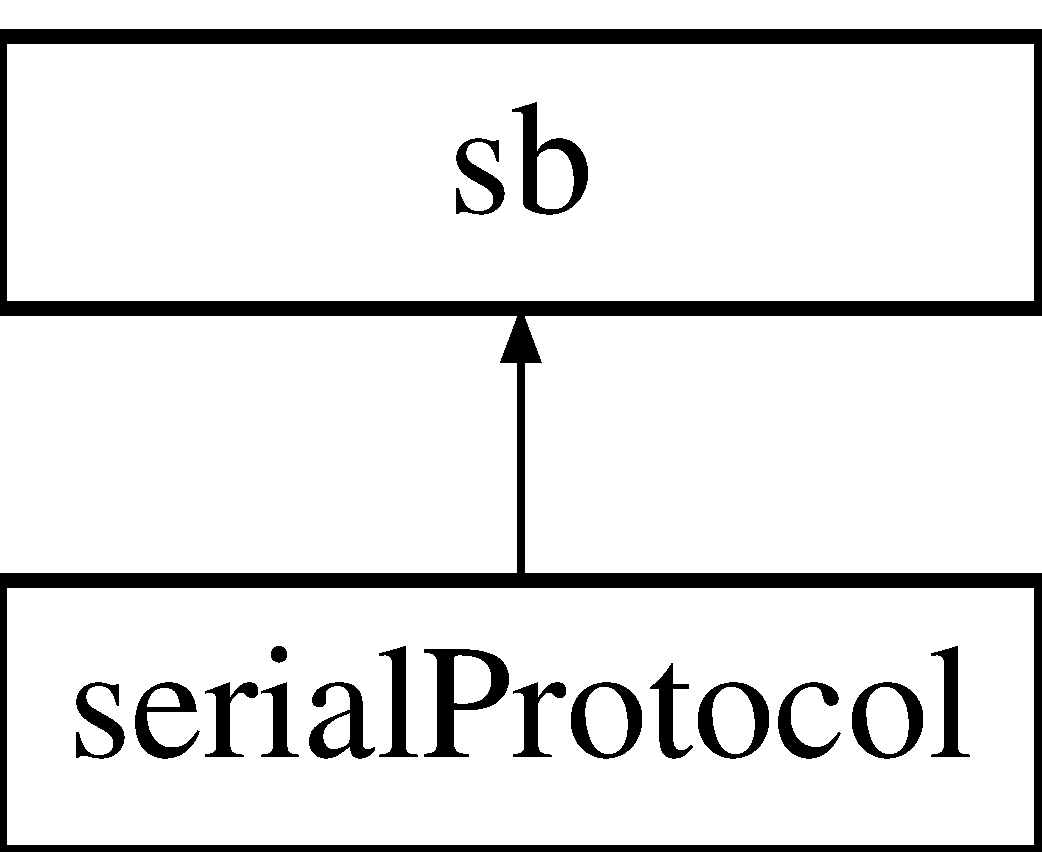
\includegraphics[height=2.000000cm]{structserial_protocol}
\end{center}
\end{figure}
\subsection*{Public Attributes}
\begin{DoxyCompactItemize}
\item 
B\+Y\+T\+E \hyperlink{structserial_protocol_af8bbcf22377b98dadf690666f9d48156}{sb}
\item 
B\+Y\+T\+E \hyperlink{structserial_protocol_a76964847a69881951e9da1317cc17571}{id}
\item 
B\+Y\+T\+E \hyperlink{structserial_protocol_a3e40b60e8c92091fb59e00ee05a07eb1}{data\+Low} \mbox{[}8\mbox{]}
\item 
B\+Y\+T\+E \hyperlink{structserial_protocol_a4f9b454d8730babf5397c1f1d582e727}{data\+High} \mbox{[}8\mbox{]}
\item 
B\+Y\+T\+E \hyperlink{structserial_protocol_aeafe645e9ba8983649aac07b5c85f1a2}{cs}
\item 
B\+Y\+T\+E \hyperlink{structserial_protocol_a75f22d859a2edf76df2fc96f8dd4b901}{cn}
\item 
B\+Y\+T\+E \hyperlink{structserial_protocol_af8e01f5811bdc9a2906aceed9ae19f0f}{eb}
\end{DoxyCompactItemize}


\subsection{Detailed Description}
use following protocol \+: S\+B$\vert$\+I\+D$\vert$\+D0...D15$\vert$\+C\+S$\vert$\+C\+N$\vert$\+E\+B 

\hyperlink{structserial_protocol}{serial\+Protocol} class. , id, data\+Low, data\+High, cs, cn, eb 

\subsection{Member Data Documentation}
\hypertarget{structserial_protocol_a75f22d859a2edf76df2fc96f8dd4b901}{}\index{serial\+Protocol@{serial\+Protocol}!cn@{cn}}
\index{cn@{cn}!serial\+Protocol@{serial\+Protocol}}
\subsubsection[{cn}]{\setlength{\rightskip}{0pt plus 5cm}B\+Y\+T\+E serial\+Protocol\+::cn}\label{structserial_protocol_a75f22d859a2edf76df2fc96f8dd4b901}
data counter, facultative ?? \hypertarget{structserial_protocol_aeafe645e9ba8983649aac07b5c85f1a2}{}\index{serial\+Protocol@{serial\+Protocol}!cs@{cs}}
\index{cs@{cs}!serial\+Protocol@{serial\+Protocol}}
\subsubsection[{cs}]{\setlength{\rightskip}{0pt plus 5cm}B\+Y\+T\+E serial\+Protocol\+::cs}\label{structserial_protocol_aeafe645e9ba8983649aac07b5c85f1a2}
Cheksum of data, maybe the mean of the 16 byte data ??? or C\+R\+C \hypertarget{structserial_protocol_a4f9b454d8730babf5397c1f1d582e727}{}\index{serial\+Protocol@{serial\+Protocol}!data\+High@{data\+High}}
\index{data\+High@{data\+High}!serial\+Protocol@{serial\+Protocol}}
\subsubsection[{data\+High}]{\setlength{\rightskip}{0pt plus 5cm}B\+Y\+T\+E serial\+Protocol\+::data\+High\mbox{[}8\mbox{]}}\label{structserial_protocol_a4f9b454d8730babf5397c1f1d582e727}
High part of the data \hypertarget{structserial_protocol_a3e40b60e8c92091fb59e00ee05a07eb1}{}\index{serial\+Protocol@{serial\+Protocol}!data\+Low@{data\+Low}}
\index{data\+Low@{data\+Low}!serial\+Protocol@{serial\+Protocol}}
\subsubsection[{data\+Low}]{\setlength{\rightskip}{0pt plus 5cm}B\+Y\+T\+E serial\+Protocol\+::data\+Low\mbox{[}8\mbox{]}}\label{structserial_protocol_a3e40b60e8c92091fb59e00ee05a07eb1}
Low part of the data -\/$>$ M\+S\+B first transmission (most significant bit) -\/$>$ transmission end when transmitting L\+S\+B bit \hypertarget{structserial_protocol_af8e01f5811bdc9a2906aceed9ae19f0f}{}\index{serial\+Protocol@{serial\+Protocol}!eb@{eb}}
\index{eb@{eb}!serial\+Protocol@{serial\+Protocol}}
\subsubsection[{eb}]{\setlength{\rightskip}{0pt plus 5cm}B\+Y\+T\+E serial\+Protocol\+::eb}\label{structserial_protocol_af8e01f5811bdc9a2906aceed9ae19f0f}
End byte \hypertarget{structserial_protocol_a76964847a69881951e9da1317cc17571}{}\index{serial\+Protocol@{serial\+Protocol}!id@{id}}
\index{id@{id}!serial\+Protocol@{serial\+Protocol}}
\subsubsection[{id}]{\setlength{\rightskip}{0pt plus 5cm}B\+Y\+T\+E serial\+Protocol\+::id}\label{structserial_protocol_a76964847a69881951e9da1317cc17571}
Identification byte \hypertarget{structserial_protocol_af8bbcf22377b98dadf690666f9d48156}{}\index{serial\+Protocol@{serial\+Protocol}!sb@{sb}}
\index{sb@{sb}!serial\+Protocol@{serial\+Protocol}}
\subsubsection[{sb}]{\setlength{\rightskip}{0pt plus 5cm}B\+Y\+T\+E serial\+Protocol\+::sb}\label{structserial_protocol_af8bbcf22377b98dadf690666f9d48156}
Start byte 

The documentation for this struct was generated from the following file\+:\begin{DoxyCompactItemize}
\item 
lib/serial\+Data.\+h\end{DoxyCompactItemize}

%--- End generated contents ---

% Index
\backmatter
\newpage
\phantomsection
\clearemptydoublepage
\addcontentsline{toc}{chapter}{Index}
\printindex

\end{document}
